\documentclass[a4paper, 12pt]{report}

\usepackage{alltt, fancyvrb, url}
\usepackage{graphicx}
\usepackage[margin=2cm]{geometry}
\usepackage[utf8]{inputenc}
\usepackage{float}
\usepackage{hyperref}
\usepackage{xurl}
\usepackage{lipsum}
\usepackage[htt]{hyphenat}
\usepackage{tabularx}
\usepackage{array}
\usepackage{color}
\usepackage{colortbl}
\usepackage[table]{xcolor}
\usepackage[font={small,it}]{caption}

\usepackage[italian]{babel}
\usepackage[italian]{cleveref}
\usepackage[toc,page]{appendix}

\definecolor{seaGreen}{cmyk}{0.19, 0, 0.25, 0.09}

\newenvironment{sloppypar*}{\sloppy\ignorespaces}{\par}

\newenvironment{changemargin}[2]{%
  \begin{list}{}{%
    \setlength{\topsep}{0pt}%
    \setlength{\leftmargin}{#1}%
    \setlength{\rightmargin}{#2}%
    \setlength{\listparindent}{\parindent}%
    \setlength{\itemindent}{\parindent}%
    \setlength{\parsep}{\parskip}%
  }%
  \item[]}{\end{list}}

\newenvironment{packed_enum}{
\begin{enumerate}
        \setlength{\itemsep}{1pt}
        \setlength{\parskip}{0pt}
        \setlength{\parsep}{0pt}
}{\end{enumerate}}

\title{Relazione Progetto Basi di Dati 2022}
\author{Michele Montesi \\
        Matricola: 0000974934 \\
        E-Mail: michele.montesi3@studio.unibo.it}

\date{\today}

\begin{document}
    
\maketitle
\tableofcontents

\chapter{Analisi Dei Requisiti}
Si vuole realizzare un database a supporto dell'automatizzazione della gestione di una
comunità la quale gestisce diverse residenze per pazienti psichiatrici.
La base di dati dovrà immagazzinare informazioni relative agli operatori, ai pazienti e
alle varie residenze.

\section{Intervista}
Un primo testo ottenuto dall'intervista è il seguente:

\begin{changemargin}{0.5cm}{0.5cm}
        \noindent
        Si vuole tenere traccia di \textbf{pazienti} e \textbf{dipendenti} memorizzandone le informazioni personali
        quali codice fiscale, nome, cognome, compleanno e sesso.
        Differenziando le due entità si memorizzeranno, inoltre, le informazioni legate alla propria posizione.
        Questi due soggetti possono essere registrati nel sistema solo accettando alcune clausole o
        disponendo di eventuali requisiti.\\
        I \textbf{dipendenti} possono acquisire degli \textbf{attestati} che gli conferiscono crediti ECM e possono firmare
        \textbf{contratti} (prima di firmare un secondo contratto con lo stesso nome, il primo deve essere concluso).
        Di entrambi verrà mantenuto uno storico.\\
        I \textbf{turni} dei dipendenti sono determinati dal codice fiscale del dipendente, il giorno della settimana, 
        l'ora d'inizio, l'ora di fine e l'unità operativa in cui si svolgeranno.\\
        I \textbf{pazienti} sono identificati da una \textbf{cartella clinica} la quale contiene informazioni riguardanti
        l'anamnesi, la diagnosi e il progetto riabilitativo del paziente. A ognuno di questi verrà assegnata una 
        \textbf{terapia} la quale dovrà essere seguita assumendo farmaci (somministrati da dipendenti) e della quale
        verrà mantenuto uno storico.\\
        I \textbf{farmaci} sono caratterizzati dal loro codice, il nome, la casa farmaceutica, le date d'acquisto e
        di scadenza e la quantità.\\
        Sono presenti \textbf{unità operative} (le quali possono essere \texttt{gruppi appartamento} o \texttt{residenze
        sanitarie psichiatriche}) adibite all' \textbf{ospitazione} di più pazienti (la quale dovrà essere registrata
        con data d'inizio e opzionalmente con una data di fine) della quale verrà mantenuto uno storico.
        Queste sono caratterizzate dalla loro ubicazione, i posti letto e il numero dei pazienti.
        Per poter essere operative devono ricevere l'\texttt{autorizzazione al funzionamento} e l'\texttt{accreditamento}.
        Ogni unità operativa avrà una lista di \textbf{beni strumentali}, i quali possono essere automezzi o attrezzature.
\end{changemargin}

\section{Estrazione dei concetti principali}\label{sec:estrazione-dei-concetti-principali}
\begin{tabularx}{\textwidth}{lXc}
        \rowcolor{seaGreen}
        \textbf{Termine} & \textbf{Breve descrizione} & \textbf{Eventuali sinonimi} \\
        Dipendente & Colui che è assunto dalla società e lavora in una o più strutture a seconda dei turni e
        somministra farmaci ai pazienti.\ Può essere socio.\ & Lavoratore \\
        \hline
        Contratto & Oggetto contenente le ore lavorative mensili del dipendente a cui viene sottoscritto.\ & Contratto Lavorativo \\
        \hline
        Attestato & Oggetto che conferisce, al dipendente che ne consegue il completamento, crediti EMC (crediti formativi).\ & Formazione \\
        \hline
        Paziente & Colui che riceve le cure attraverso la somministrazione di farmaci, seguendo una terapia, ed è ospitato
        all'interno di una unità operativa.\ & Cliente \\
        \hline
        Cartella clinica & Documentazione del paziente contenente anamnesi, diagnosi e progetto riabilitativo.\ & Cartella \\
        \hline
        Terapia & Oggetto che riporta i farmaci da assumere durante un periodo di tempo.\ & Cura \\
        \hline
        Farmaco & Medicinale adibito all'assunzione da parte di pazienti a cui è stato assegnato.\ & Medicinale \\
        \hline
        Unità operativa & Residenza o appartamento i cui i pazienti risiedono e ricevono le cure da parte del personale.\ & Residenza, Unità \\
        \hline
        Bene strumentale & Strumento o veicolo aziendale necessario o utile a semplificare il lavoro o la permanenza nell'unità operativa.\ & Strumentazione, Veicolo
\end{tabularx}
\\\\\\
A seguito della lettura e comprensione dei requisiti, si procede redigendo un testo che ne 
riassuma tutti i concetti e in particolare ne estragga quelli principali eliminando le ambiguità 
sopra rilevate:

\begin{changemargin}{0.5cm}{0.5cm}
        \noindent
        Per ogni \textbf{dipendente} vengono memorizzati Codice Fiscale, Nome, Cognome, Compleanno, Residenza, Sesso, Titolo di Studio,
        l'Idoneità alla mansione, se è Socio o meno e i Crediti ECM. Ogni dipendente dispone, inoltre, di un codice univoco fornitogli
        al momento del suo inserimento nel DB. 
        Ogni dipendente può acquisire degli \textbf{attestati} che gli conferiscono crediti ECM e possono firmare
        \textbf{contratti} (prima di firmare un secondo contratto con lo stesso nome, il primo deve essere concluso).
        Di entrambi verrà mantenuto uno storico.\\
        I \textbf{turni} dei dipendenti sono determinati dal codice fiscale del dipendente, il giorno della settimana, 
        l'ora d'inizio, l'ora di fine e l'unità operativa in cui si svolgeranno. Un turno di uno stesso dipendente nello stesso
        giorno della settimana non potrà essere definito se si interseca ad un altro.\\
        Per ogni \textbf{paziente} vengono memorizzati Codice Fiscale, Nome, Cognome, Compleanno, Residenza, Sesso.
        Al momento della registrazione dovrà firmare la documentazione alla privacy, il consenso al trattamento e l'accettazione
        del regolamento. Ognuno possiede una \textbf{cartella clinica} la quale contiene informazioni riguardanti
        l'anamnesi, la diagnosi e il progetto riabilitativo. A ognuno di questi verrà assegnata una 
        \textbf{terapia} la quale dovrà essere seguita assumendo farmaci (somministrati da dipendenti) e della quale
        verrà mantenuto uno storico.\\
        Ogni \textbf{farmaco} è caratterizzato dal loro codice, il nome, la casa farmaceutica, le date d'acquisto e
        di scadenza e la quantità.\\
        Ogni \textbf{unità operativa} può essere \texttt{gruppo appartamento} o \texttt{residenza sanitaria psichiatrica}.
        Ognuna di queste è adibita all' \textbf{ospitazione} di più pazienti (la quale dovrà essere registrata
        con data d'inizio e opzionalmente con una data di fine) della quale verrà mantenuto uno storico.
        Ognuna è caratterizzate dall'ubicazione, i posti letto e il numero dei pazienti.
        Per poter essere operative devono ricevere l'\texttt{autorizzazione al funzionamento} e l'\texttt{accreditamento}.
        Ogni unità operativa avrà una lista di \textbf{beni strumentali}, i quali possono essere automezzi o attrezzature.
        \newline
\end{changemargin}
Segue un elenco delle principali operazioni richieste:
\begin{packed_enum}
        \item Registrare un nuovo dipendente
        \item Registrare un turno
        \item Registrare un nuovo paziente
        \item Registrare un farmaco
        \item Registrare una nuova unità operativa
        \item Registrare un contratto
        \item Registrare un attestato
        \item Assegnare un contratto ad un dipendente
        \item Assegnare un attestato ad un dipendente
        \item Far assumere un farmaco ad un paziente
        \item Visualizzare tutti i dipendenti
        \item Visualizzare tutti i pazienti
        \item Visualizzare tutti i turni
\end{packed_enum}

\chapter{Progettazione Concettuale}

\section{Schema scheletro}
Le entità di \textbf{dipendente} e \textbf{paziente} sono la generalizzazione di una entità \textbf{persona}, identificata
tramite il codice fiscale. Dall'analisi del dominio si evince come serva tenere uno storico di tutti i farmaci somministrati
da un dipendente ad un paziente. Perciò si reifica l'associazione tra \textbf{dipendente} e \textbf{terapia} generando
una nuova entità \textbf{farmaco\_terapia} che tiene traccia della quantità del \textbf{farmaco} somministrato, la data, 
il somministratore e la terapia. Questa entità è definita dal suo \textit{codice univoco incrementale}, il \textit{codice della terapia} ed 
il \textit{codice del dipendente}.

\begin{figure}[H]
        \centering
        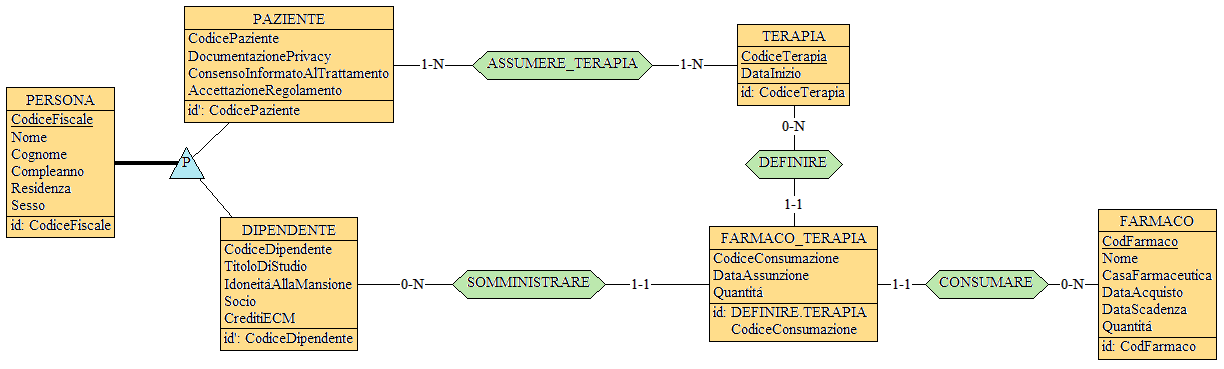
\includegraphics[height=5cm]{img/dipendentePazienteER.png}
        \caption{Schema E/R con le principali entità per modellazione della somministrazione di farmaci}
    \end{figure}

\section{Schema finale}

\chapter{Progettazione Logica}

\section{Stima del volume dei dati}


\end{document}